% !TeX root = ../thuthesis-example.tex

\chapter{数据集分析与对比}
\section{开源数据集}
% \subsection{UNSW-NB15}
流量异常检测领域的开源数据集要么过于久远,无法反映当前的网络环境,要么模拟访问环境过于简单,可信度很低。因此流量异常检测领域的高质量的开源数据集很少。本文采用目前应用最为广泛的两个数据集,UNSW-NB15和CICDIS2017,尽管这两个数据集也有很多不足。
澳大利亚网络安全中心(ACCS)的网络范围实验室在KDD99数据集的基础上,生成了UNSW-NB15数据集\cite{moustafa2015unsw}的原始网络流量数据。该数据集主要利用IXIA PerfectStorm工具生成正常活动的流量和人为构造的多种攻击流量。相比于陈旧的KDD99数据集\cite{ozgur2016review},其更能代表真实的网络流量。

CICIDS2017数据集是由加拿大网络安全研究所(Canadian Institute for Cybersecurity)提供。与UNWS-NB15类似,CICIDS2017也是在仿真环境中模拟正常流量和攻击流量生成的。

UNSW-NB15的实验环境划分了3个子网,采用了45个独立的ip地址,持续约30个小时,采集了共100GB的原始网络流量数据。CICIDS2017的实验环境划分了2个子网,分为受害者子网和攻击者子网,受害者子网共有12台主机,攻击者子网共4台主机,累计测量时间持续约5天,共采集了51.1GB的pcap流量数据。由这两者的实验环境可以看出,开源数据集在规模上远远无法和真实流量环境对比。

% 该数据集包括 100GB的.pcap 格式的原始网络流量,具有九种攻击类型,分别是Fuzzers,Analysis,Backdoors,DoS,Exploits,Generic,Reconnaissance,Shellcode和Worms。每种攻击的具体描述和类别数目如表所示。该数据集还包含4个经过特征提取的csv文件,一共2540044 条数据。


% UNSW-NB15 数据集一共包含 47 个特征,其中时间戳,IP 地址,端口号等特征对训练无用,因此有效的特征一共 41 个。 
% 下面对这些特征做一个概括的说明。按照数据集作者的思路,可以分为基本
% 特征,内容特征,时间特征和额外生成的特征这几类。

以UNSW-NB15为例,图\ref{fig:UNSW-NB15数据集生成过程}展示了该数据集的生成过程。首先,通过使用Tcupdump工具监测访问环境中的流量情况,生成pcap文件;然后使用Argus\footnote{https://qosient.com/argus/index.shtml}和Bro-IDS\footnote{https://www.bro.org/index.html}工具从报文信息中直接提取基于数据包和数据流的特征,并根据五元组(源ip地址,源端口号,目的ip地址,目的端口号,协议类型)信息进行匹配,此时基本特征、内容特征和时间特征已生成;接下来为了能够更有效地识别攻击,还需要额外生成一些统计特征。最终将这些特征保存成csv文件。



这些数据集生成流程和特征提取方法给后续我们分析清华大学校园网的流量数据提供了参考。


\begin{figure}
    \centering
    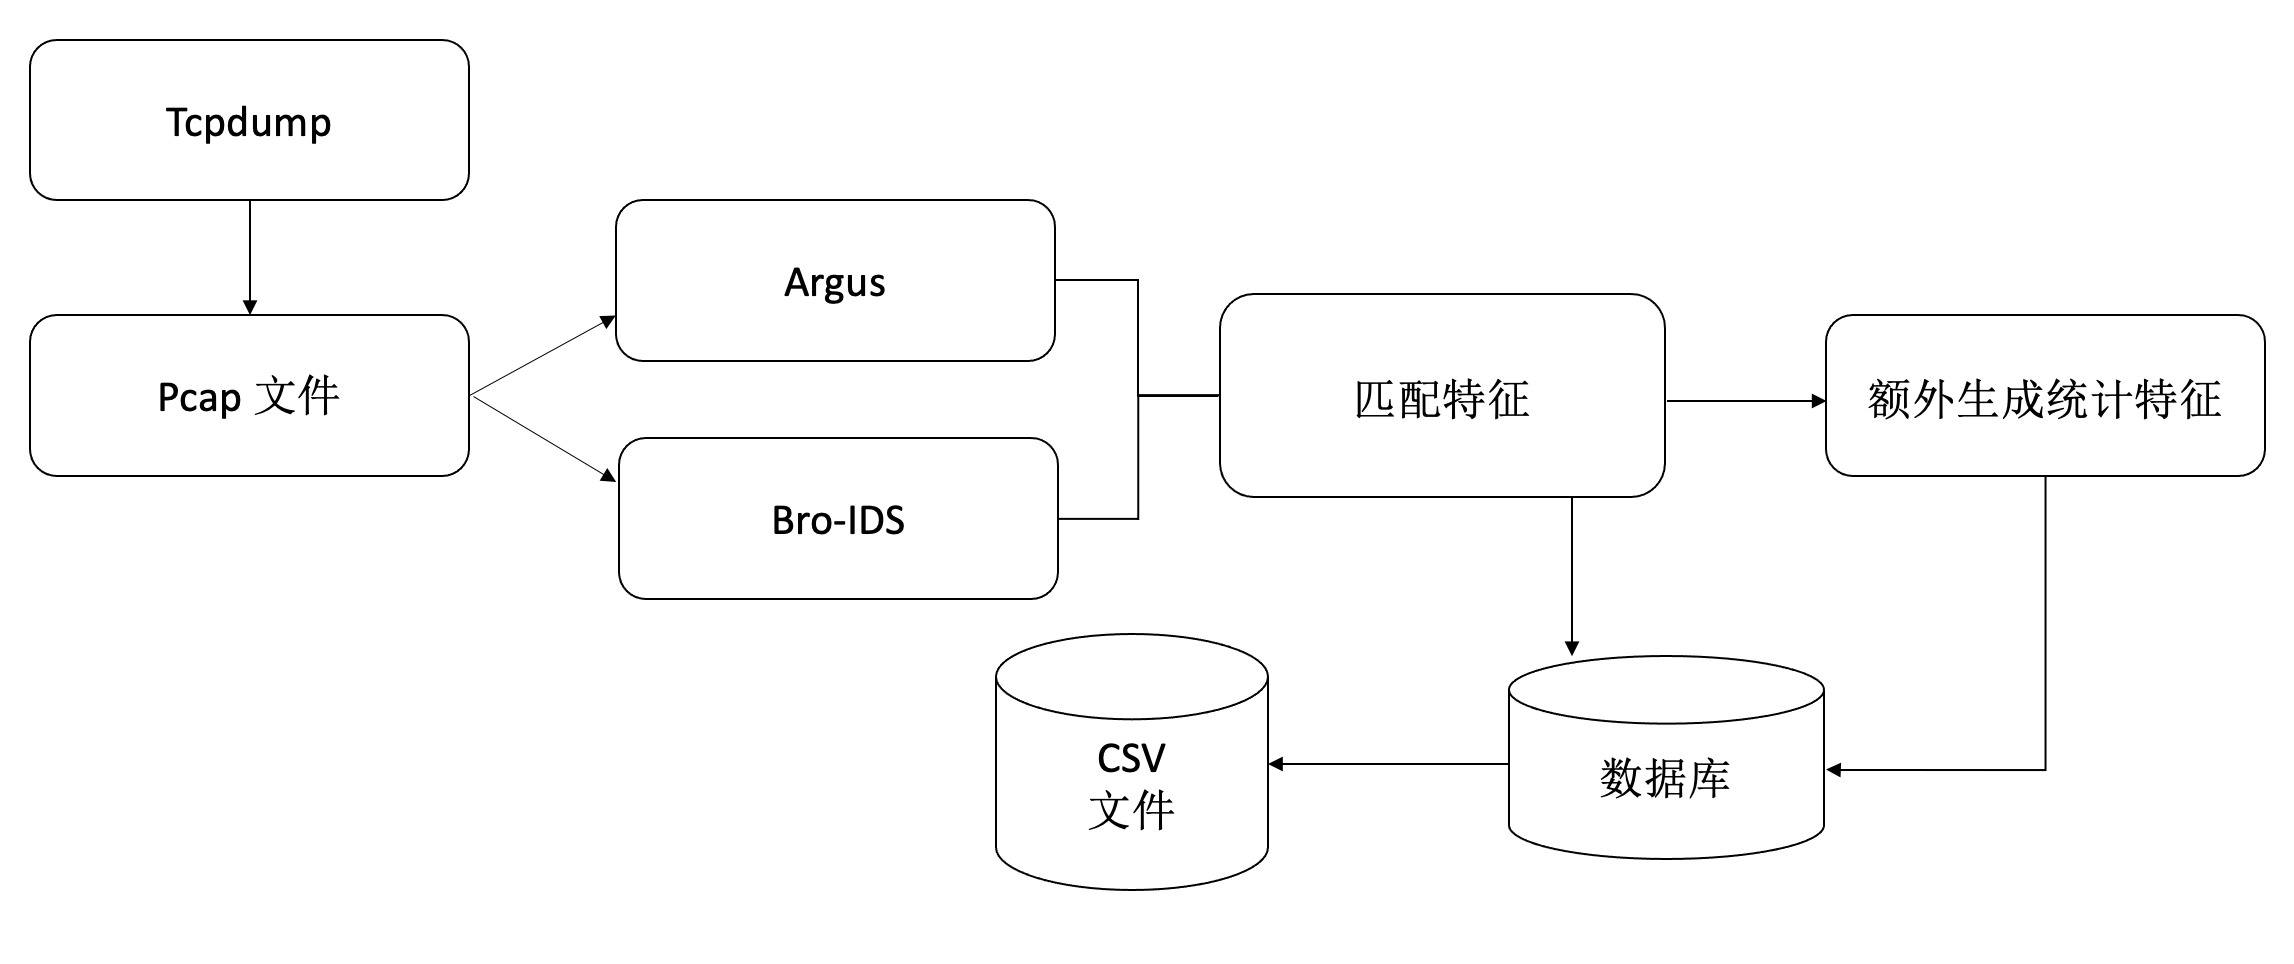
\includegraphics[width=0.6\linewidth]{UNSW-NB15 framework.png}
    \caption{UNSW-NB15数据集生成过程}
    \label{fig:UNSW-NB15数据集生成过程}
  \end{figure}

% \begin{table}[H]
%     \caption{UNSW-NB15数据集攻击类别}
%     \begin{tabular}{p{0.18\linewidth}<{\raggedright} | p{0.6\linewidth}<{\raggedright}| p{0.12\linewidth}<{\raggedright}}
%     % \begin{tabular}{|p{0.2\columnwidth}<{\centering} |p{0.7\textwidth}<{\centering} |p{0.1\textwidth}<{\centering}|}
%     % \begin{tabular}{lp{3cm}p{9cm}p{3cm}}
%     \toprule 
%     类别 & 类别描述                                                                       & 样本数量    \\ \midrule 
%     Normal  & 正常流量                                                                       & 2218761 \\ \hline
%     Fuzzers & 攻击者从命令行或以报文的形式发送大量随机生成的输入序列。攻击者试图发现操作系统、程序或网络中的安全漏洞,并使这些资源挂起一段时间,甚至可以使它们崩溃。 & 24246   \\ \hline
%     Analysis & 这类攻击是指通过端口扫描、恶意 web 脚本
% (如 HTML 文件渗透)和发送垃圾邮件等各种
% 方式渗透到 web 应用程序的各种入侵等。 & 2677 \\ \hline
% Backdoor & 这类攻击中攻击者可以绕过正常的身份验证
% 并获得对系统的未授权远程访问。黑客利用
% 后门程序安装恶意文件,修改代码或获得对
% 系统或数据的访问。 &
% 2329 \\ \hline
% DoS & 攻击者使某些计算或内存资源过于繁忙或占
% 据全部资源而无法处理合法请求或者拒绝合
% 法用户对计算机的访问。 &
% 16353 \\ \hline
% Exploit & 利用操作系统或软件中的软件漏洞、漏洞或
% 故障进行入侵的行为。攻击者利用软件的知
% 识发动攻击,意图对系统造成危害。 &
% 44525 \\ \hline
% Generic & 针对密码系统的攻击,试图破坏安全系统的
% 密钥。它独立于密码系统的实现细节。不考
% 虑块密码的结构。例如,生日攻击是一种将
% 哈希函数视为黑盒的通用攻击。 &
% 215481 \\ \hline
% Reconnaissance & 为了绕过目标计算机网络的安全控制而收集
% 其信息的攻击。它可以被定义为一个探针,
% 是发起进一步攻击的初步步骤。攻击者使用
% 各种扫描手段来收集系统信息。在收集到足
% 够的信息后,可以发起后续的攻击。 &
% 13987 \\ \hline
% Shellcode & Shellcode 作为负载在目标机器执行,来挖掘
% 该软件的漏洞。之所以称作 Shellcode 是因为
% 启动了受到攻击者控制的命令行 shell。 &
% 1511 \\ \hline
% Worm & 蠕虫是一种恶意程序或恶意软件,它可以复
% 制自己并传播到其他计算机。 &
% 174 \\  
% \bottomrule
% \end{tabular}
% \label{label:UNSW-NB15}
% \end{table}

% \begin{table}[H]
%     \caption{基本特征}
%     \label{基本特征}
%     \centering
%     \begin{tabular}{|l|l|}
%         \toprule
%         特征名称 & 特征描述 \\
%         \midrule
%         state & 会话的状态和相应的协议 \\
%         dur & 会话的持续时间 \\
%         sbytes & 会话中从源发出的总字节数 \\
%         dbytes & 会话中从目的发出的总字节数 \\
%         sttl & 从源发出的报文的 time to live \\
%         dttl & 从目的发出的报文的 time to live 字段 \\
%         sloss & 源的丢包数和重传数之和 \\
%         dloss & 目的的丢包数和重传数之和 \\
%         service & 应用层协议 \\
%         sload & 源报文的吞吐量 \\
%         dload & 目的报文的吞吐量 \\
%         spkts & 会话中源的报文总数 \\
%         dpkts & 会话中目的报文总数 \\
%         \bottomrule
%     \end{tabular}
% \end{table}

% \begin{table}[H]
%     \caption{内容特征}
%     \label{内容特征}
%     \centering
%     \begin{tabular}{|l|l|}
%         \toprule
%         特征名称 & 特征描述 \\
%         \midrule
%         swin & 源 tcp 报文的窗口字段 \\
%         dwin & 目的 tcp 报文的窗口字段 \\
%         stcpb & 源 tcp 报文的初始序列号 \\
%         dtcpb & 目的 tcp 报文的初始序列号 \\
%         smeansz & 会话中源报文的平均大小 \\
%         dmeansz & 会话中目的报文的平均大小 \\
%         trans\_depth & http 服务的连接深度 \\
%         res\_bdy\_len & http 响应内容的长度 \\
%         \bottomrule
%     \end{tabular}
% \end{table}

% \begin{table}
%     \caption{时间特征}
%     \label{时间特征}
%     \centering
%     \begin{tabular}{|l|l|}
%         \toprule
%         特征名称 & 特征描述 \\
%         \midrule
%         sjit & 源报文间隔时间的标准差(jitter) \\
%         djit & 目的报文间隔时间的标准差 \\
%         stime &  报文开始时间\\
%         ltime &  报文结束时间\\
%         sintpkt & 源报文的间隔时间的平均值 \\
%         dintpkt & 目的报文间隔时间的平均值 \\
%         tcprtt & tcp 三次握手的 rtt(round trip time) \\
%         synack & 第一次发送到确认的时间 \\
%         ackdat & 确认之后返回的时间 \\
%         \bottomrule
%     \end{tabular}
% \end{table}

% \begin{table}
%     \caption{额外生成的统计特征}
%     \label{额外生成的统计特征}
%     \centering
%     \begin{tabular}{l|p{0.7\textwidth}<{\centering}}
%         \toprule
%         特征名称 & 特征描述 \\
%         \midrule
%         is\_sm\_ips\_ports & 源 ip 与目的 ip,源端口和目的端口是否都相同 \\
%         ct\_state\_ttl  & 对于每一个状态,ttl 值的范围 \\
%         ct\_flw\_http\_mthd & 在http服务中具有GET和POST方法的会话计数  \\
%         is\_ftp\_login  & 是否有 ftp 的登录 \\
%         ct\_ftp\_cmd  & 会话中 ftp 命令的计数 \\
%         ct\_srv\_src  & 根据最后一条报文的时间排序,每 100 条记录中源ip 与服务都相同的会话计数(下面省略每 100 条) \\
%         ct\_srv\_dst  & 目的 IP 与服务都相同的会话计数 \\
%         ct\_dst\_ltm  & 目的 IP 相同的会话计数 \\
%         ct\_src\_ltm  & 源 IP 相同的会话计数 \\
%         ct\_src\_dport\_ltm  & 源 IP 和目的端口都相同的会话计数 \\
%         ct\_dst\_sport\_ltm  & 目的 IP 和源端口都相同的会话计数 \\
%         ct\_dst\_src\_ltm  & 目的 IP 和源 IP 都相同的会话计数 \\
%         \bottomrule
%     \end{tabular}
% \end{table}




% \begin{table}[H]
%     \caption{与协议相关的特征}
%     \centering
%     \begin{tabular}{l|l}
%     \hline
%     特征名称                  & 特征描述                      \\ \hline
%     proto                 & 传输层协议                     \\ \hline
%     service               & 应用层协议                     \\ \hline
%     sttl                  & 从源发出的报文的 time to live     \\ \hline
%     dttl                  & 从目的发出的报文的 time to live 字段 \\ \hline
%     stcpb                 & 源 tcp 报文的初始序列号            \\ \hline
%     dtcpb                 & 目的 tcp 报文的初始序列号           \\ \hline
%     swin                  & 源 tcp 报文的窗口字段             \\ \hline
%     dwin                  & 目的 tcp 报文的窗口字段            \\ \hline
%     res\_bdy\_len         & http 响应内容的长度              \\ \hline
%     ct\_flw\_http\_method & 会话中 http 方法字段的计数          \\ \hline
%     is\_ftp\_login        & 是否有 ftp 的登录               \\ \hline
%     ct\_ftp\_cmd          & 会话中 ftp 命令的计数             \\ \hline
%     trans\_depth          & http 服务的连接深度              \\ \hline
%     \end{tabular}
%     \end{table}

% \begin{table}[H]
%     \caption{与时间相关的特征}
%     \centering
%     \begin{tabular}{|l|l|}
%     \hline
%     dur     & 会话的持续时间                        \\ \hline
%     tcprtt  & tcp 三次握手的 rtt(round trip time) \\ \hline
%     synack  & 第一次发送到确认的时间                    \\ \hline
%     ackdat  & 确认之后返回的时间                      \\ \hline
%     sintpkt & 源报文的间隔时间的平均值                   \\ \hline
%     dintpkt & 目的报文间隔时间的平均值                   \\ \hline
%     sjit    & 源报文间隔时间的标准差(jitter)            \\ \hline
%     djit    & 目的报文间隔时间的标准差                   \\ \hline
%     sload   & 源报文的吞吐量                        \\ \hline
%     dload   & 目的报文的吞吐量                       \\ \hline
%     \end{tabular}
%     \end{table}

%     \begin{table}[H]
%         \caption{与报文大小相关的特征}
%         \centering
%         \begin{tabular}{|l|l|}
%         \hline
%         sbytes  & 会话中从源发出的总字节数  \\ \hline
%         dbytes  & 会话中从目的发出的总字节数 \\ \hline
%         smeansz & 会话中源报文的平均大小   \\ \hline
%         dmeansz & 会话中目的报文的平均大小  \\ \hline
%         spkts   & 会话中源的报文总数     \\ \hline
%         dpkts   & 会话中目的报文总数     \\ \hline
%         \end{tabular}
%         \end{table}

% \begin{table}[H]
%     \caption{与连接状态相关的特征}
%     \centering
%     \begin{tabular}{|l|l|}
%     \hline
%     sloss & 源的丢包数和重传数之和  \\ \hline
%     dloss & 目的的丢包数和重传数之和 \\ \hline
%     state & 会话的状态和相应的协议  \\ \hline
%     \end{tabular}
%     \end{table}

% \begin{table}[H]
%     \caption{额外构造的特征}
%     \centering
%     \begin{tabular}{|l|p{0.7\textwidth}<{\centering}|}
%     \hline
%     ct\_srv\_src                & 根据最后一条报文的时间排序,每 100 条记录中源ip 与服务都相同的会话计数(下面省略每 100 条)  \\ \hline
%     ct\_srv\_dst                & 目的 IP 与服务都相同的会话计数         \\ \hline
%     ct\_dst\_ltm                & 目的 IP 相同的会话计数             \\ \hline
%     ct\_src\_ltm                & 源 IP 相同的会话计数              \\ \hline
%     ct\_src\_dport\_ltm         & 源 IP 和目的端口都相同的会话计数        \\ \hline
%     ct\_dst\_sport\_ltm         & 目的 IP 和源端口都相同的会话计数        \\ \hline
%     ct\_dst\_src\_ltm           & 目的 IP 和源 IP 都相同的会话计数      \\ \hline
%     ct\_state\_ttl              & 对于每一个状态,ttl 值的范围          \\ \hline
%     is\_sm\_ips\_ports          & 源 ip 与目的 ip,源端口和目的端口是否都相同 \\ \hline
%     \end{tabular}
%     \end{table}


% \subsection{CICIDS2017}
% CICIDS2017数据集是由加拿大网络安全研究所(Canadian Institute for Cybersecurity)提供。与UNWS-NB15类似,CICIDS2017也是在仿真环境中模拟正常流量和攻击流量生成的。
% CICIDS数据集特征介绍如下:(修改格式,解释表格)


% List of extracted features and descriptions: \\


% \begin{table}[H]
%     \caption{packet大小相关的特征}
%     \centering
%     \begin{tabular}{|l|l|}
%     \hline
%     total Length of Fwd Packet	& 发送方packet总长度 \\
%     total Length of Bwd Packet	& 接收方packet总长度 \\
%     Fwd Packet Length Min 		& 发送方packet最小长度 \\
%     Fwd Packet Length Max 		& 发送方packet最大长度 \\
%     Fwd Packet Length Mean		& 发送方packet平均长度 \\
%     Fwd Packet Length Std		& 发送方packet长度标准差 \\
%     Bwd Packet Length Min		& 接收方packet最小长度 \\
%     Bwd Packet Length Max		& 接收方packet最大长度 \\
%     Bwd Packet Length Mean		& 接收方packet平均长度 \\
%     Bwd Packet Length Std		& 接收方packet长度标准差 \\
%     \hline
%     \end{tabular}
%     \end{table}

% \begin{table}[H]
%     \caption{时间相关的特征}
%     \centering
%     \begin{tabular}{|l|l|}
%     \hline
%     Flow Bytes/s		&	bps \\
%     Flow Packets/s		&	pps  \\
%     Flow IAT Mean		&	一条流中包平均间隔时间 \\
%     Flow IAT Std		&	一条流中包间隔时间的标准差 \\
%     Flow IAT Max		&	一条流中两个packet最大间隔时间 \\
%     Flow IAT Min		&	一条流中两个packet最小间隔时间 \\
%     Fwd IAT Min			&发送方两个packet最小间隔时间\\
%     Fwd IAT Max			&发送方两个packet最大间隔时间 \\
%     Fwd IAT Mean		&	发送方两个packet平均间隔时间 \\
%     Fwd IAT Std			&发送方两个packet间隔时间的标准差 \\
%     Fwd IAT Total   	&	发送方两个packet总间隔时间\\
%     Bwd IAT Min			&接收方两个packet最小间隔时间\\
%     Bwd IAT Max			&接收方两个packet最大间隔时间\\
%     Bwd IAT Mean		&	接收方两个packet平均间隔时间 \\
%     Bwd IAT Std			&接收方两个packet间隔时间的标准差 \\
%     Bwd IAT Total		&	接收方两个packet总间隔时间 \\  
%     \hline
%     \end{tabular}
%     \end{table}
% \begin{table}
%     \caption{标志位相关的特征}
%     \centering
%     \begin{tabular}{|l|l|}
%     \hline
%     Fwd PSH flags		&	发送方PSH标志位出现次数(0 for UDP) \\
%     Bwd PSH Flags		&	接收方PSH标志位出现次数(0 for UDP)\\
%     Fwd URG Flags		&	发送方URG标志位出现次数(0 for UDP) \\
%     Bwd URG Flags		&	接收方URG标志位出现次数(0 for UDP) \\
%     FIN Flag Count 		&	FIN标志位出现次数 \\
%     SYN Flag Count 		&	SYN标志位出现次数 \\
%     RST Flag Count 		&	RST标志位出现次数 \\
%     PSH Flag Count 		&	PUSH标志位出现次数 \\
%     ACK Flag Count 		&	ACK标志位出现次数 \\
%     URG Flag Count 		&	URG标志位出现次数 \\
%     CWR Flag Count 		&	CWR标志位出现次数 \\
%     ECE Flag Count 		&	ECE标志位出现次数 \\
%     \hline
%     \end{tabular}
% \end{table}
    
% Flow duration  单条流持续时间/微秒 \\
% total Fwd Packet		发送方packet数量 \\
% total Bwd packets		接收方packet数量 \\


% Fwd Header Length		发送方header占用的总字节数 \\
% Bwd Header Length		接受方header占用的总字节数 \\
% FWD Packets/s			发送方pps \\
% Bwd Packets/s			接收方pps \\
% Packet Length Min 		packet最小长度 \\
% Packet Length Max		packet最大长度 \\
% Packet Length Mean 		packet平均长度 \\
% Packet Length Std		packet长度标准差 \\
% Packet Length Variance  	packet长度方差 \\

% down/Up Ratio			下载/上传比 \\
% Average Packet Size 		packet平均大小 \\
% Fwd Segment Size Avg 		发送方数据块平均大小?\\
% Bwd Segment Size Avg 		接收方数据块平均大小?\\
% Fwd Bytes/Bulk Avg		Average number of bytes bulk rate in the forward direction \\
% Fwd Packet/Bulk Avg		Average number of packets bulk rate in the forward direction \\
% Fwd Bulk Rate Avg 		Average number of bulk rate in the forward direction \\
% Bwd Bytes/Bulk Avg		Average number of bytes bulk rate in the backward direction \\
% Bwd Packet/Bulk Avg 		Average number of packets bulk rate in the backward direction \\
% Bwd Bulk Rate Avg		Average number of bulk rate in the backward direction \\
% Subflow Fwd Packets		The average number of packets in a sub flow in the forward direction \\
% Subflow Fwd Bytes		The average number of bytes in a sub flow in the forward direction \\
% Subflow Bwd Packets		The average number of packets in a sub flow in the backward direction \\
% Subflow Bwd Bytes		The average number of bytes in a sub flow in the backward direction \\
% Fwd Init Win bytes		The total number of bytes sent in initial window in the forward direction \\
% Bwd Init Win bytes		The total number of bytes sent in initial window in the backward direction \\
% Fwd Act Data Pkts		Count of packets with at least 1 byte of TCP data payload in the forward direction \\
% Fwd Seg Size Min		Minimum segment size observed in the forward direction \\
% Active Min			Minimum time a flow was active before becoming idle \\
% Active Mean			Mean time a flow was active before becoming idle \\
% Active Max			Maximum time a flow was active before becoming idle \\
% Active Std			Standard deviation time a flow was active before becoming idle \\
% Idle Min			Minimum time a flow was idle before becoming active \\
% Idle Mean			Mean time a flow was idle before becoming active \\
% Idle Max			Maximum time a flow was idle before becoming active \\
% Idle Std			Standard deviation time a flow was idle before becoming active \\

\section{校园网流量数据集}
清华大学无线网规模巨大,具有超过6万名日活跃用户,13万个可用ip地址,是全球最大的校园无线网之一。通过出口网关的服务器我们可以得到海量的真实流量数据,但是这与可进行分析和训练的数据集之间还有巨大的鸿沟。因此本节参考图\ref{fig:UNSW-NB15数据集生成过程}中的数据集生成流程,结合UNSW-NB15和CICIDS2017两个数据集中特征的特点,生成了校园网的特征数据集。校园网数据集制作流程如图\ref{fig:流量数据集制作流程}所示。首先将pcap流量数据切分成多个会话(session,双向流中所有的数据包),依次从每个会话中提取报文信息以及统计信息构成特征;然后以五元组作为流的标识符,把从SOC平台中得到的告警信息与特征信息合并起来,就生成了最终的数据集。
\begin{figure}
    \centering
    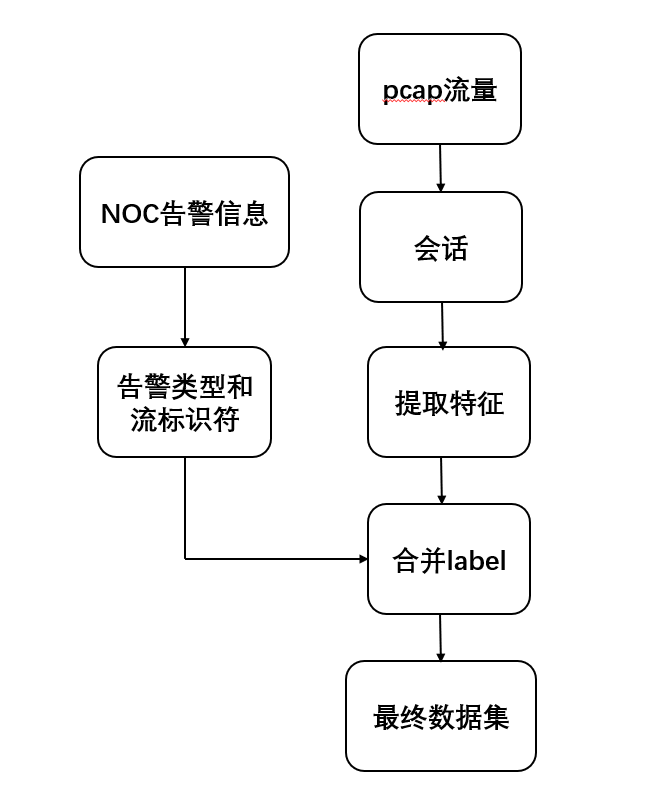
\includegraphics[scale=0.6]{流量数据集制作流程.png}
    % 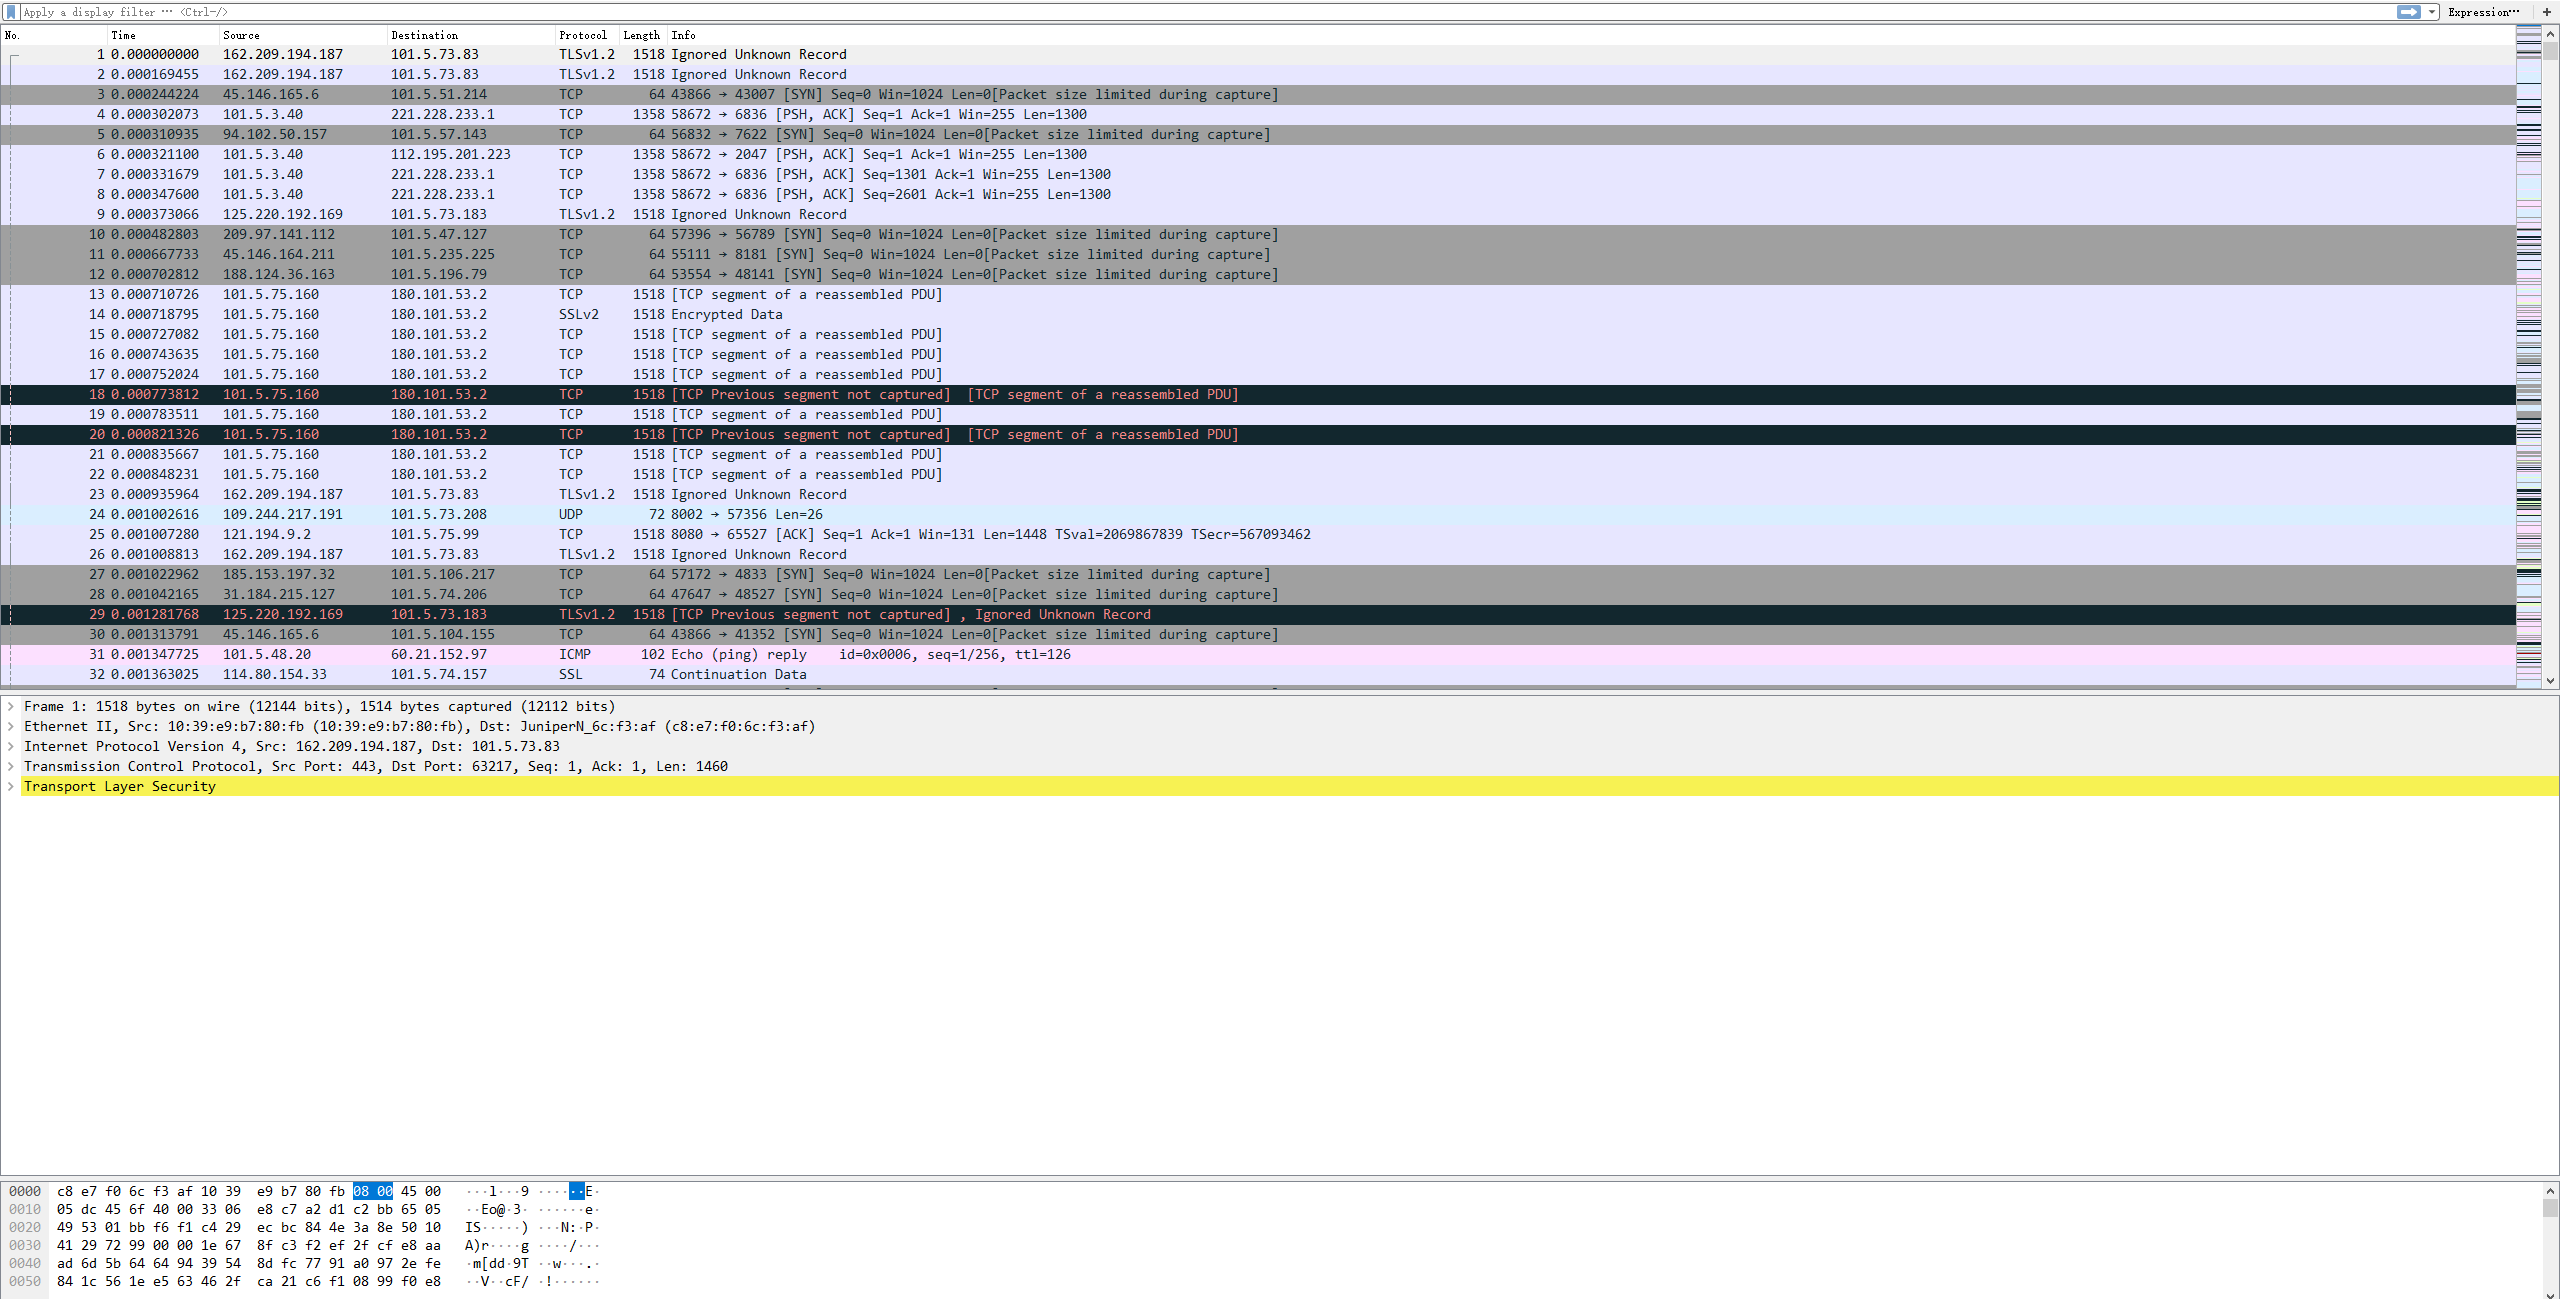
\includegraphics[width=0.6\linewidth]{wireshark流量图.png}
    \caption{流量数据集制作流程}
    \label{fig:流量数据集制作流程}
  \end{figure}


本节共采集了两类数据集,分别是出口网关处的全流量数据、安全管理平台(Security Operations Center,SOC)的威胁告警日志。
接下来分别介绍这四类数据。

\subsection{全流量日志数据}
校园网的原始数据为抓包(Packet Capture,pcap)流量,如下图~\ref{fig:wireshark}所示,其中包含每个数据包的详细信息,如五元组、报文头部信息、报文内容等,本文对所有用户隐私信息(如IP地址和MAC地址,报文中的明文信息等)都进行了匿名化处理,保证不会泄露用户的任何隐私信息。

\begin{figure}
    \centering
    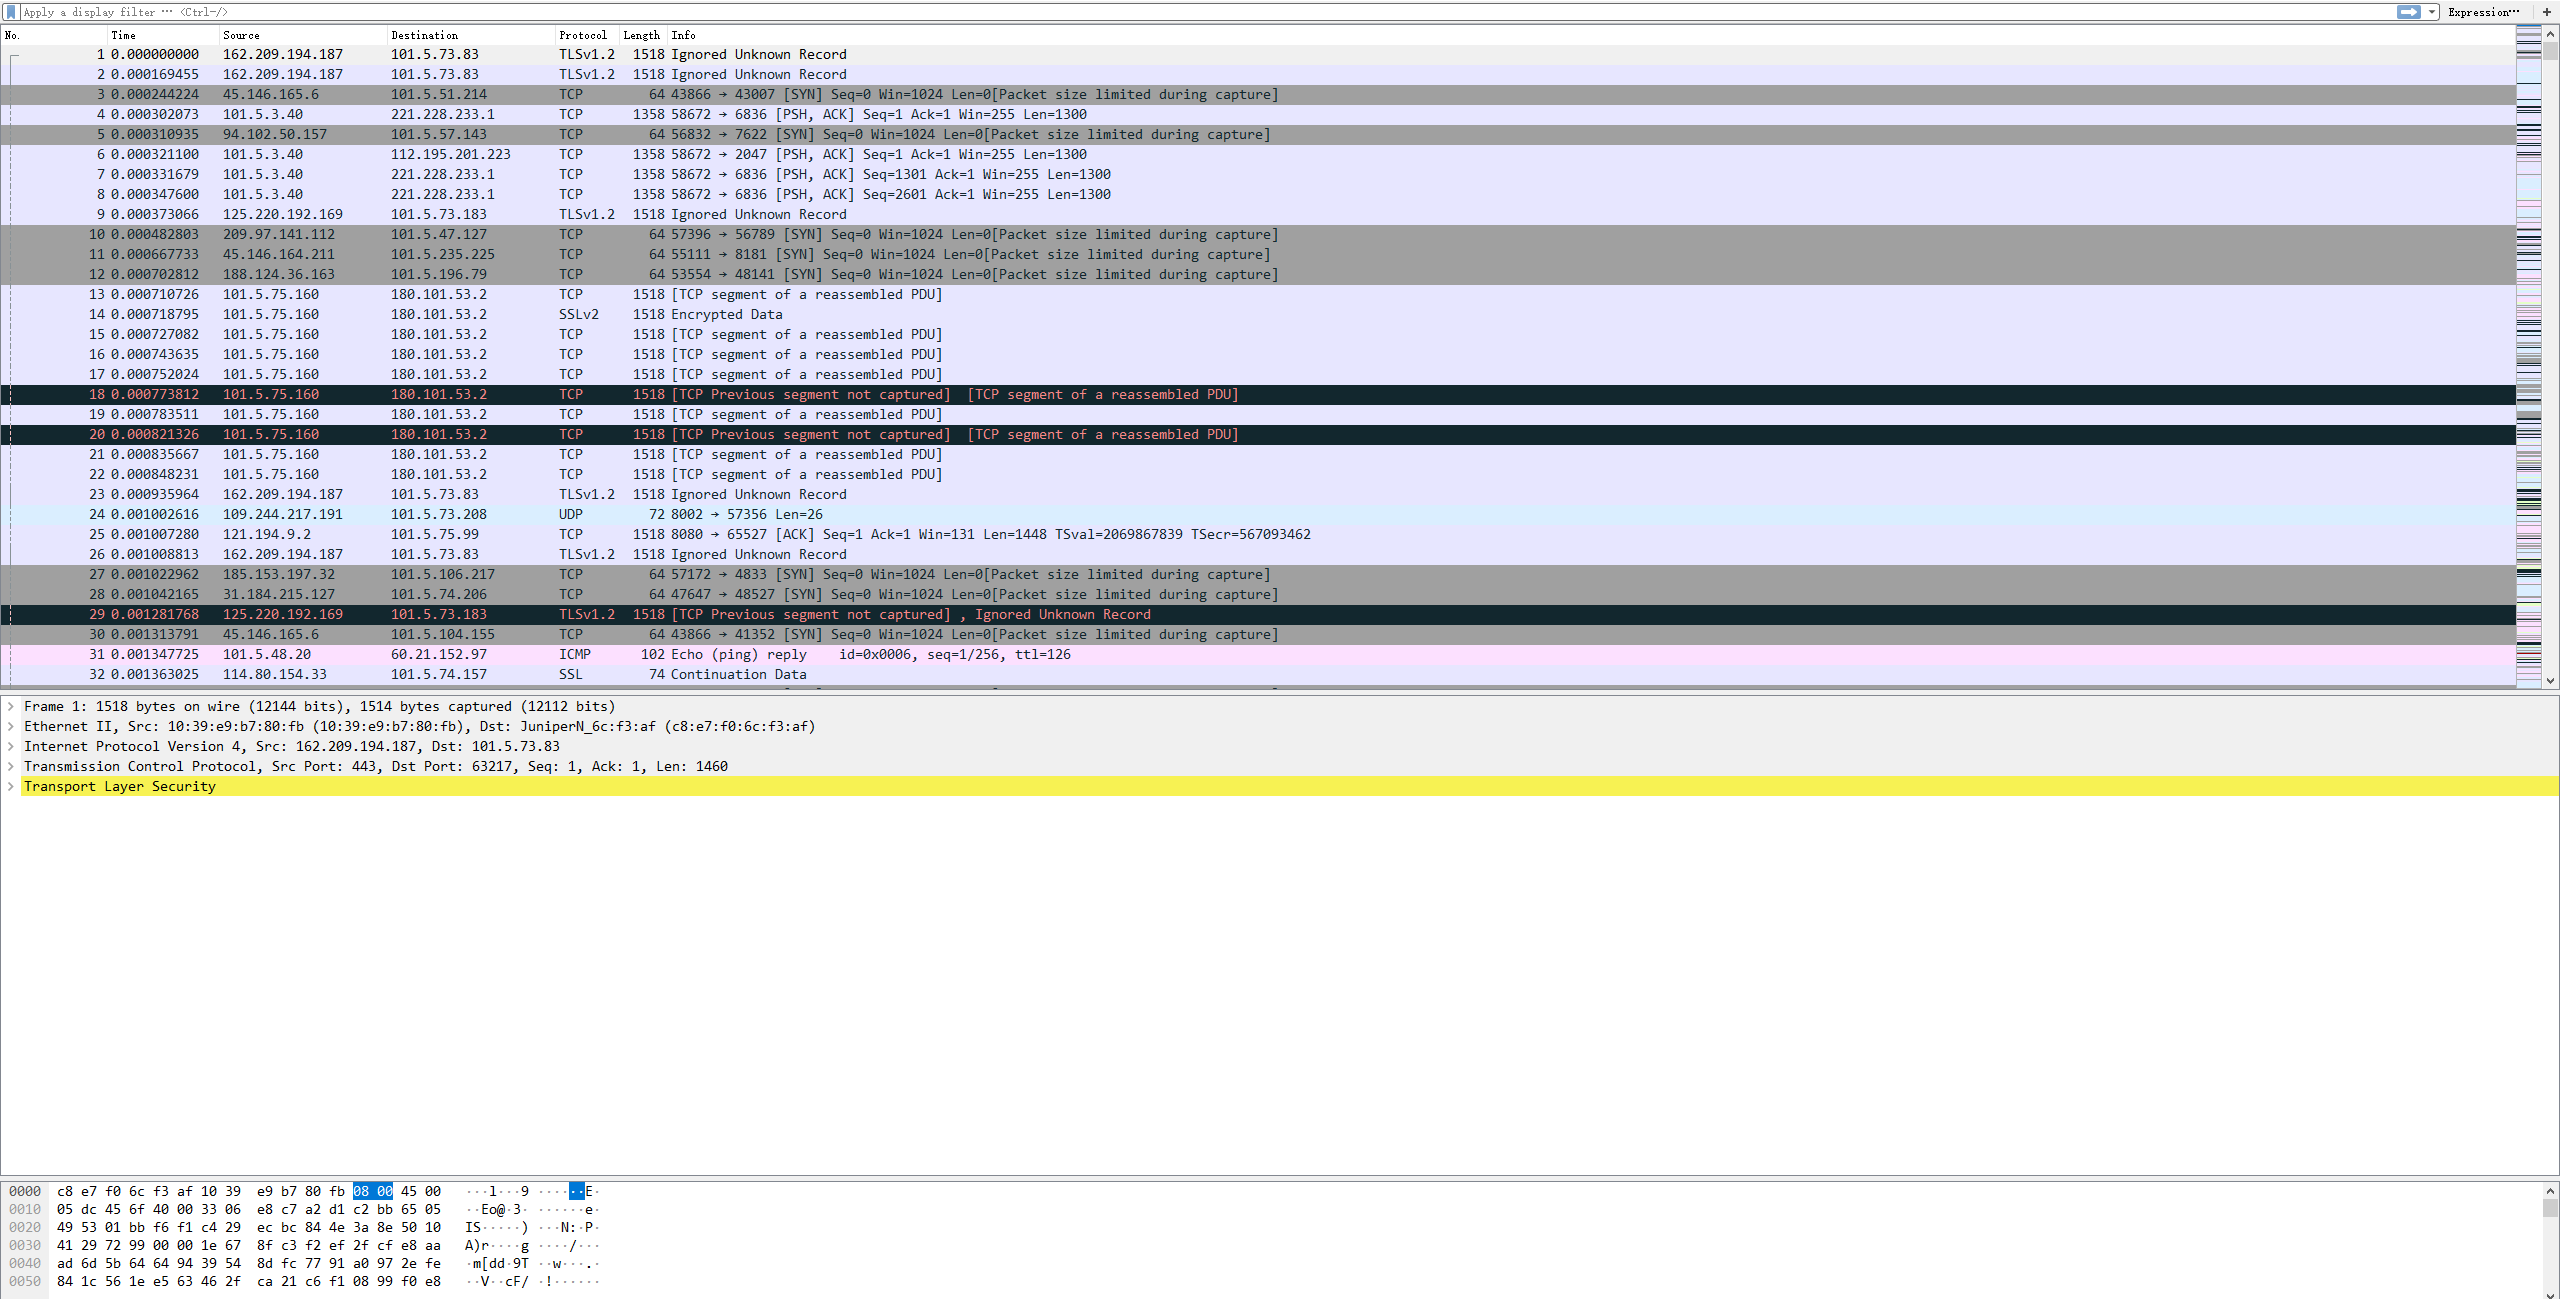
\includegraphics[scale=0.22]{wireshark流量图.png}
    \caption{流量数据示意图}
    \label{fig:wireshark}
  \end{figure}

%   对于机器学习模型来说,通常
%   不是直接对原始的流量进行检测,而是通过对流量提取特征,得到样本的特征向
%   量后进行检测和分类。


\subsection{威胁告警日志}
我们通过全流量日志得到了特征数据集,但是由于缺乏标注,该数据集无法进行训练以及验证。因此为了得到可进行训练的有效数据集,我们还需要对特征数据集添加标注。标注数据是根据现有的SOC平台得到,需要进行数据清洗、数据预处理等步骤。图\ref{fig:NOC平台数据样例}为NOC平台的数据样例。
\begin{figure}
    \centering
    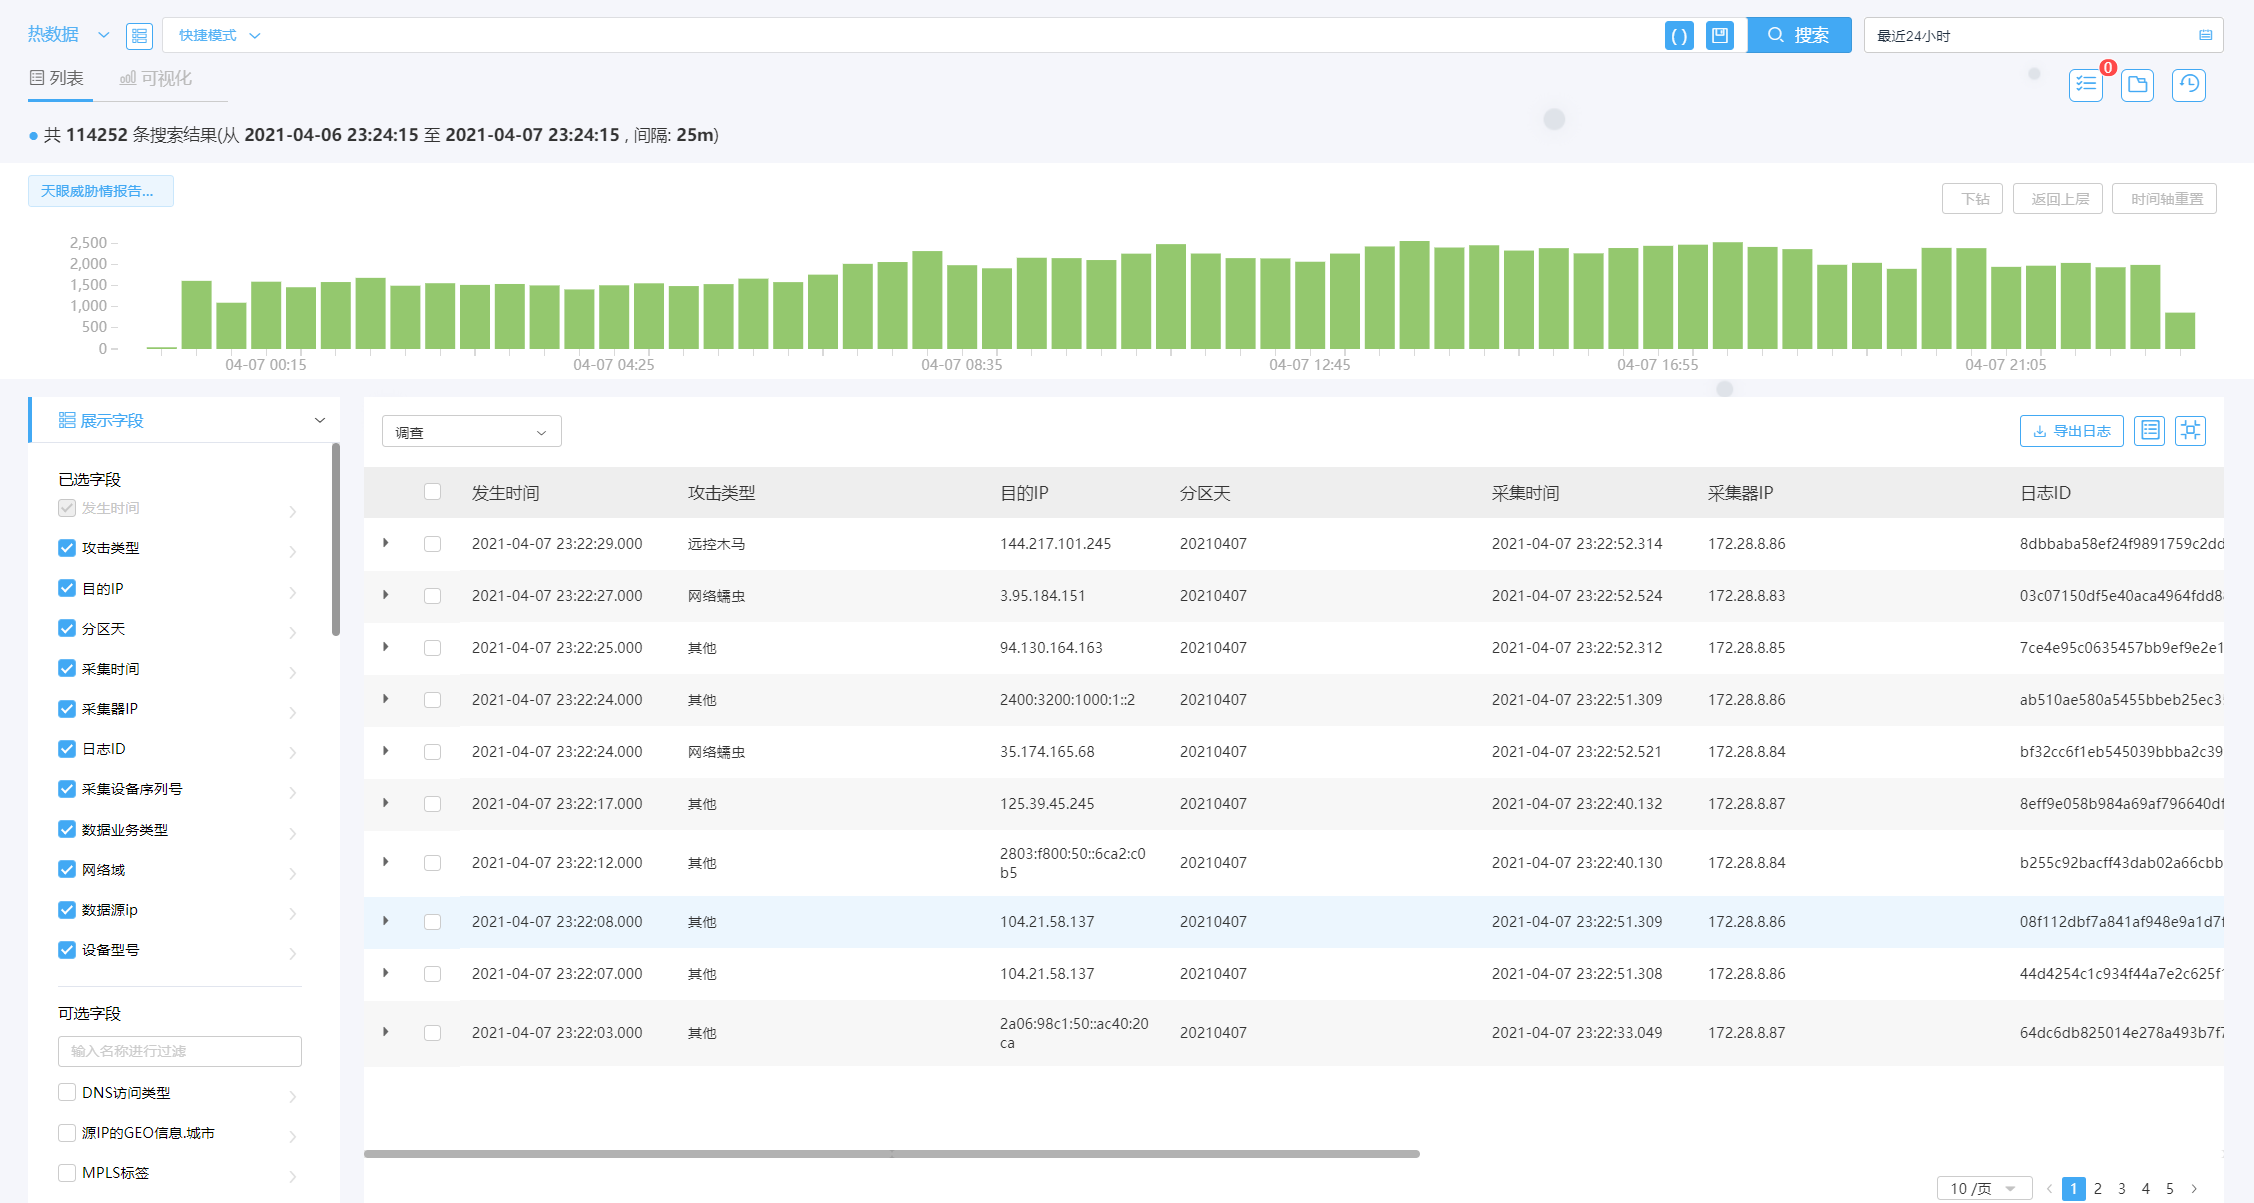
\includegraphics[scale=0.35]{NOC平台.png}
    \caption{NOC平台数据样例}
    \label{fig:NOC平台数据样例}
  \end{figure}
% \subsection{TCP流量和UDP流量日志}

% \subsection{数据预处理及评价指标}
% 得到特征数据集后,通常仍然无法直接进行训练,因为其中可能包含非法值、无效值、字符串值等,需要对数据进行预处理。首先是对数据进行清洗,删除掉不必要的噪声数据、非法数据,将无效值进行填充。
% 后续操作总结如下:

% 1. 删除套接字信息:由于原始数据集包含网络中源主机和目标主机的 IP 地址和端口号,因此删除这些信息以提供无偏检测非常重要,使用这些信息可能会导致对该套接字信息的过度训练。

% 2. 删除空格:数据集中的一些多类标签包含空格。由于实际值不同于同一
% 类中其他元组的标签,因此这些空白会导致不同的类。

% 3. 标签编码:数据集中的多个类标签都有攻击的名称,即字符串值。因此
% 这些值编码成数值是很重要的,分类器就可以学习每个元组所属的类号。

% 4. 数据规范化:数据集中的数值数据属于不同的范围,这给分类器在训练
% 过程中补偿这些差异带来了一些挑战。因此,规范化每个属性中的值很重要,这
% 样,每个属性中的最小值为零,而最大值为一。这为分类器提供了更均匀的值,
% 同时保持了每个属性值之间的相关性。

% 在实验中,本论文使用四个指标来评估模型的性能:准确率,精确度,召回
% 率和 $F1-score$。对于一个数据样本检测的结果可分为下面的结果:

% \begin{enumerate}
%     \item TP:入侵网络流量被入侵检测正确的识别为入侵网络流量。
%     \item TN:正常网络流量被入侵检测正确的识别为正常网络流量。
%     \item FN:入侵网络流量被入侵检测错误的识别为正常网络流量。
%     \item FP:正常网络流量被入侵检测错误的识别成入侵网络流量。
% \end{enumerate}

% % 1. TP:入侵网络流量被入侵检测正确的识别为入侵网络流量

% % 2. TN:正常网络流量被入侵检测正确的识别为正常网络流量

% % 3. FN:入侵网络流量被入侵检测错误的识别为正常网络流量

% % 4. FP:正常网络流量被入侵检测错误的识别成入侵网络流量

% 论文使用下面的方法去评估我们提出方法的性能:
% 准确率(Accuracy): 预测正确的样本的数量与所有被预测样本数量的比值,
% 公式如下 所示。
% \begin{equation}
%     Accuracy = \frac{TP + TN}{TP + TN + FN + FP}
% \end{equation}

% 精确度(Precision): 这个指标于分类器衡量的被错误分类的数量所惩罚的
% 正确分类的数量,公式如 下所示:
% \begin{equation}
%     Precision = \frac{TP}{TP + FP}
% \end{equation}
% 召回率(Recall): 针对样本而言的表示的是数据正样本中有多少被预测正
% 确。这种度量反映了分类器检测网络攻击的能力,公式如下  所示:
% \begin{equation}
%     Recall = \frac{TP}{TP+ FN}
% \end{equation}
% $F1-score$:此调和平均值这是用以计量精确度以及召回率的,可以平衡的反映算法的精确度,公式如下所示:
% \begin{equation}
%     F1-score = 2*\frac{Precision * Recall}{Precision + Recall}
% \end{equation}

\section{现有算法在不同数据集的评估}
本节分别在以上三个数据集上进行实验,对比了现有的经典算法,以下是这些算法的名称、特点及实验中的参数。


待补充结果对比图


\begin{table*}[t]
    \small
    \caption{部分评估结果,待填充具体数值}
    \label{table2}
    \centering
    \begin{tabular}{c|c|ccc|ccc|cc}
    \toprule
    
     数据集 &  任务  &  
     LR &  NB & DT & CNN & CNN-LSTM & GRU & DCRNN-A & DCRNN-B \\
    \midrule
    % & 5\% & 79.87 & 80.61 & 79.08 & 81.69 & 78.05 & 75.80 & 82.21 & \textbf{82.49}\\
    
    % & 4\% &79.35 & 80.22 & 78.89 & 80.85 & 75.07 & 72.41 & 82.11 & \textbf{82.44} \\
    
    UNSW-NB15 & 二分类 & 0.848 & 79.33 & 78.52 &  80.51 & 62.74 & 68.91 & \textbf{82.69} & 81.66 \\ 
    
    & 多分类 &76.73 & 77.96 & 76.82 & 77.98 & 47.11 & 56.30 & \textbf{81.05} & 79.94 \\
    
    % & 1\% & 66.58 & 70.09 & 68.18 & 71.23 & 32.95 & 46.71 & \textbf{71.76} & 71.62 \\
    \midrule
    % & 5\%& 70.55 & 69.41 & 68.40 &  71.45 & 70.72 & 65.11 & 71.24 &  \textbf{71.89} \\
    % & 4\% & 69.11 & 68.33& 67.13 & 70.37 & 70.41 & 64.61 & 69.74 & \textbf{71.10} \\
    NSL-KDD & 二分类 & 68.26 & 67.11 & 65.54 & 70.18 & 65.04 & 58.49 & 70.26 & \textbf{70.88} \\
    & 多分类 & 67.01 & 67.37 & 66.41 & 68.31 & 56.16 & 53.18 & 68.47 & \textbf{70.24} \\
    % & 1\% & 60.08 & 61.39 & 61.25 & 63.25 & 30.28 & 49.57 & 62.21 & \textbf{64.91} \\
    \midrule
    % & 0.5\%& 82.18 & 80.01 & 81.32 &  78.25 & \textbf{82.73} & 78.97 & 82.17 & 80.70\\
    % & 0.4\%& 80.85 & 79.09 & 79.82 & 76.32 & 81.53 &  75.86 & \textbf{81.70} & 79.92\\
    CAMPUS & 二分类 & 79.98 & 77.95 & 79.51 & 75.62 & 79.80 & 75.25 & \textbf{80.69} & 79.10\\
    & 多分类 & 76.33 & 77.01 & 77.54 & 73.01 & 76.59 & 59.28 & 78.12 & \textbf{78.89}\\
    % & 0.1\% & 69.21 & 70.99 & 71.42 & 67.92 & 42.46 & 55.92 & 72.23 & \textbf{73.17}\\
    
     \bottomrule
    
    \end{tabular}
    \end{table*}
